%%%%%%%%%%%%%%%%%%%%%%%%%%%%%%%%%%%%%%%%%%%%%%%%%%%%%%%%%%%
% --------------------------------------------------------
% Rho
% LaTeX Template
% Version 2.1.1 (01/09/2024)
%
% Authors: 
% Guillermo Jimenez (memo.notess1@gmail.com)
% Eduardo Gracidas (eduardo.gracidas29@gmail.com)
% 
% License:
% Creative Commons CC BY 4.0
% --------------------------------------------------------
%%%%%%%%%%%%%%%%%%%%%%%%%%%%%%%%%%%%%%%%%%%%%%%%%%%%%%%%%%%

\documentclass[9pt,a4paper,twoside]{rho-class/rho}
\usepackage[english]{babel}
\usepackage{amsmath}
% \usepackage{algorithmic} % Añade esto en el preámbulo
\usepackage{algorithm}
\usepackage{algpseudocode}
\usepackage{hyperref} % Para manejar URLs
\usepackage{biblatex} % Para el manejo de bibliografía

\addbibresource{rho.bib} 

%% Spanish babel recomendation
% \usepackage[spanish,es-nodecimaldot,es-noindentfirst]{babel}

\setbool{rho-abstract}{true} % Set false to hide the abstract
\setbool{corres-info}{false} % Set false to hide the corresponding author section

%----------------------------------------------------------
% TITLE
%----------------------------------------------------------

\journalname{Trabajo Final}
\title{ Quad Tree: Una Estructura de Datos Espacial. }

%----------------------------------------------------------
% AUTHORS AND AFFILIATIONS
%----------------------------------------------------------

% \author[1]{Alberto Valentín Velásquez Santos}
% \author[2]{Rodolfo Morocho Caballero}
% \author[3]{Max Houston Ramirez Martel}
% \author[4]{Harold Mondragon Tavara}
\author[,$\dagger$]{Alberto Valentín Velásquez Santos}
\author[,$\dagger$]{Rodolfo Morocho Caballero}
\author[,$\dagger$]{Max Houston Ramirez Martel}
\author[,$\dagger$]{Harold Mondragon Tavara}

%----------------------------------------------------------

% \affil[1]{Alberto Valentín Velásquez Santos}
% \affil[2]{Rodolfo Morocho Caballero}
% \affil[3]{Max Houston Ramirez Martel}
% \affil[4]{Harold Mondragon Tavara}
\affil[$\dagger$]{Estos autores contribuyeron igualmente a este trabajo.}
%----------------------------------------------------------
% DATES
%----------------------------------------------------------

\dates{Este archivo fue compilado el 09 de Marzo del 2025}

%----------------------------------------------------------
% FOOTER INFORMATION
%----------------------------------------------------------

\leadauthor{Group The Bankers}
\footinfo{Creative Commons CC BY 4.0}
\smalltitle{\LaTeX\ Template}
\institution{Universidad de Tecnologia E Ingeniería}
\theday{March 09, 2025} %\today

%----------------------------------------------------------
% ARTICLE INFORMATION
%----------------------------------------------------------

% \corres{Provide the corresponding author information and publisher here.}
% \email{example@organization.com.}
% \doi{\url{https://www.doi.org/exampledoi/XXXXXXXXXX}}

\received{March 09, 2025}
\revised{March 09, 2025}
\accepted{March 09, 2025}
\published{March 09, 2025}
\license{Rho LaTeX Class \ccLogo\ This document is licensed under Creative Commons CC BY 4.0.}

%----------------------------------------------------------
% ABSTRACT
%----------------------------------------------------------

\begin{abstract}
    Este trabajo presenta un análisis detallado del algoritmo Quad Tree, una estructura de datos jerárquica especializada en la subdivisión recursiva de espacios bidimensionales en cuadrantes. El Quad Tree permite organizar y acceder eficientemente a datos espaciales, ofreciendo una complejidad logarítmica en operaciones como búsqueda, inserción y eliminación. A lo largo del documento, se exploran sus fundamentos teóricos, su implementación computacional y sus principales aplicaciones prácticas.
    La implementación de un Quad Tree se basa en la representación de nodos que contienen información sobre coordenadas espaciales y referencias a nodos hijos correspondientes a los cuadrantes NW, NE, SW y SE. Se detallan algoritmos específicos para operaciones fundamentales como inserción y búsqueda, incluido el manejo de casos especiales como puntos ubicados en las líneas divisorias de los cuadrantes.
    Entre las aplicaciones destacadas se encuentra la detección de bordes en imágenes, donde el Quad Tree facilita la segmentación mediante un proceso de tres fases: suavizado jerárquico, clasificación por clustering y refinamiento de bordes. Otra aplicación significativa es la detección de colisiones en entornos bidimensionales, donde el Quad Tree reduce la complejidad computacional de $O(n^2)$ a $O(n \log n)$ al permitir verificar colisiones solo entre objetos ubicados en el mismo cuadrante o en cuadrantes adyacentes.
    Esta estructura de datos resulta particularmente valiosa en campos como gráficos por computadora, sistemas de información geográfica y procesamiento de imágenes, donde la eficiencia en el manejo de grandes volúmenes de datos espaciales es crucial.
\end{abstract}

%----------------------------------------------------------
\keywords{Quad Tree, Estructura de datos jerárquica, Subdivisión espacial, Detección de bordes, Detección de colisiones, Complejidad computacional, Procesamiento de imágenes}
%----------------------------------------------------------

\begin{document}
	
%----------------------------------------------------------
% OPTIMIZATION PROBLEMS
%---------------------------------------------------------- 
    \maketitle
    \section{Introducción}

        \rhostart{L}os algoritmos de particionamiento espacial son fundamentales en el campo de la computación para organizar y manipular datos geométricos de manera eficiente. Entre estas estructuras destaca el Quad Tree, una herramienta esencial que ha revolucionado el manejo de información espacial en múltiples dominios de aplicación.
        El Quad Tree representa una aproximación jerárquica para la organización de datos bidimensionales, basada en el principio de "divide y vencerás". Esta estructura subdivide recursivamente un espacio en cuatro cuadrantes iguales, creando una representación en árbol donde cada nodo puede tener exactamente cuatro hijos. Esta característica permite que las operaciones de búsqueda, inserción y eliminación se realicen con una complejidad logarítmica respecto al número de elementos, superando significativamente a las estructuras de datos lineales tradicionales.
        En el presente trabajo exploraremos en profundidad el algoritmo Quad Tree desde sus fundamentos teóricos hasta sus implementaciones prácticas. Analizaremos su estructura fundamental, los métodos de operación y las técnicas de optimización que lo hacen tan valioso. Especial atención merecen sus aplicaciones en áreas como el procesamiento de imágenes, donde facilita la detección de bordes y la segmentación, y en entornos interactivos como videojuegos, donde permite una detección de colisiones altamente eficiente.
        Los avances en hardware y la creciente demanda de aplicaciones que procesan grandes volúmenes de datos espaciales han renovado el interés por estas estructuras. Comprender las ventajas y limitaciones de los Quad Trees resulta esencial para ingenieros y científicos de datos que trabajan con representaciones espaciales y buscan optimizar el rendimiento de sus sistemas sin sacrificar la precisión en los resultados.

    \section{ Conceptos Fundamentales }
    El algoritmo Quad Tree es una estructura de datos jerárquica que permite la subdivisión recursiva de un espacio bidimensional en cuadrantes más pequeños, este método permite organizar y acceder eficientemente a los datos, facilitando operaciones en aplicaciones como gráficos por computadora, sistemas de información geográfica y procesamiento de imágenes.
    \begin{figure}[h]
        \centering
        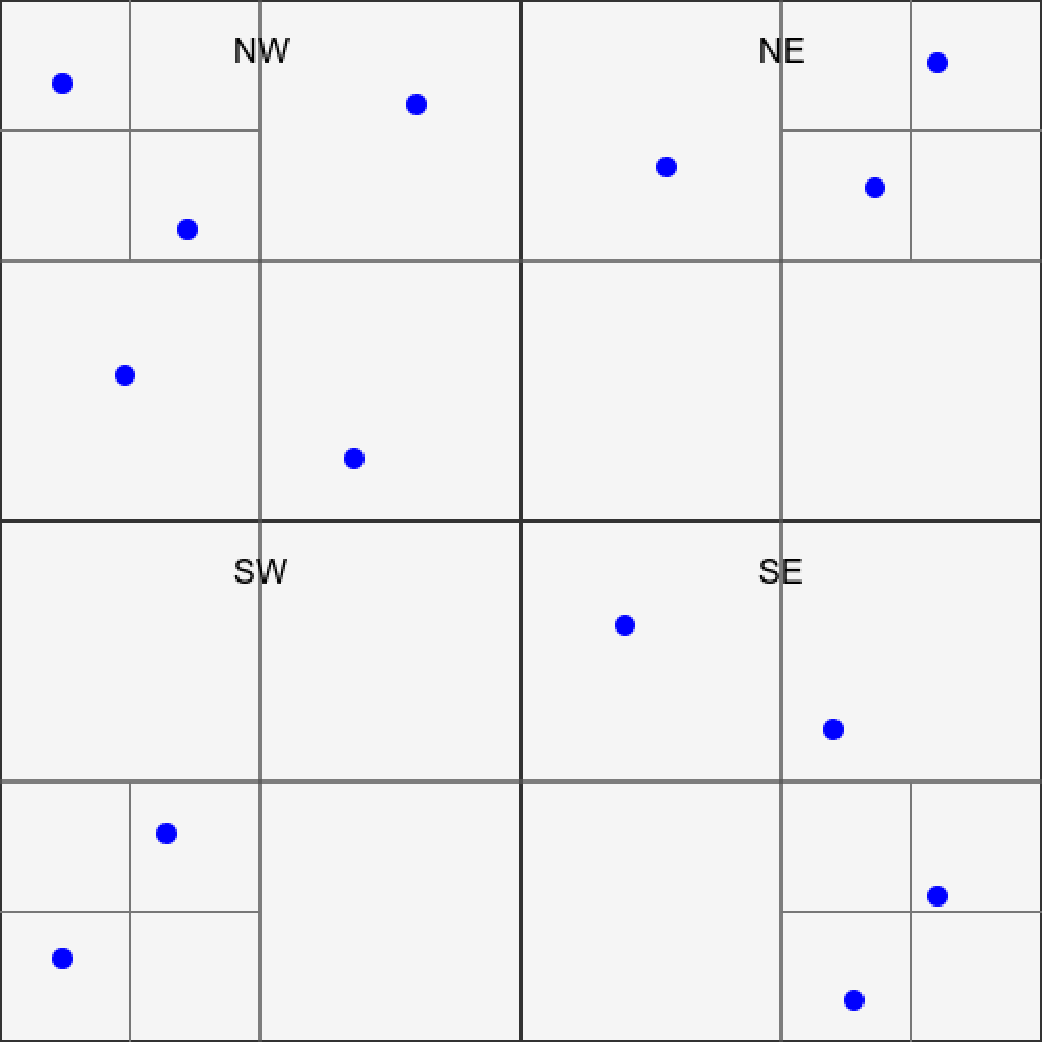
\includegraphics[width=\linewidth]{figures/quadtree.pdf}
        \caption{Representación grafica del cuadrante Quad Tree}
        \label{fig:representation_figure}
    \end{figure}\\
        \subsection{Fundamentos}
            Quad Tree tiene como principio fundamental la idea de \textit{divide y vencerás}, donde un problema complejo se descompone en subproblemas más fáciles de manipular y calcular, durante el proceso de división, este continúa hasta que se cumple una condición específica, como alcanzar una profundidad máxima o contener un número mínimo de elementos en una región.
            Matemáticamente, esta estructura permite una representación jerárquica del espacio, lo que facilita operaciones como búsqueda, inserción y eliminación de datos espaciales. La subdivisión recursiva en cuadrantes permite que las operaciones de búsqueda tengan una complejidad logarítmica en relación con el número de elementos, mejorando la eficiencia en comparación con estructuras de datos lineales, en otras palabras, se puede obtener mayor beneficio en términos de procesamiento, sin requerir tantas prestaciones en hardware y más rápido que otros algoritmos convencionales. \cite{samet_quadtree}
            \begin{figure}[h]
                \centering
                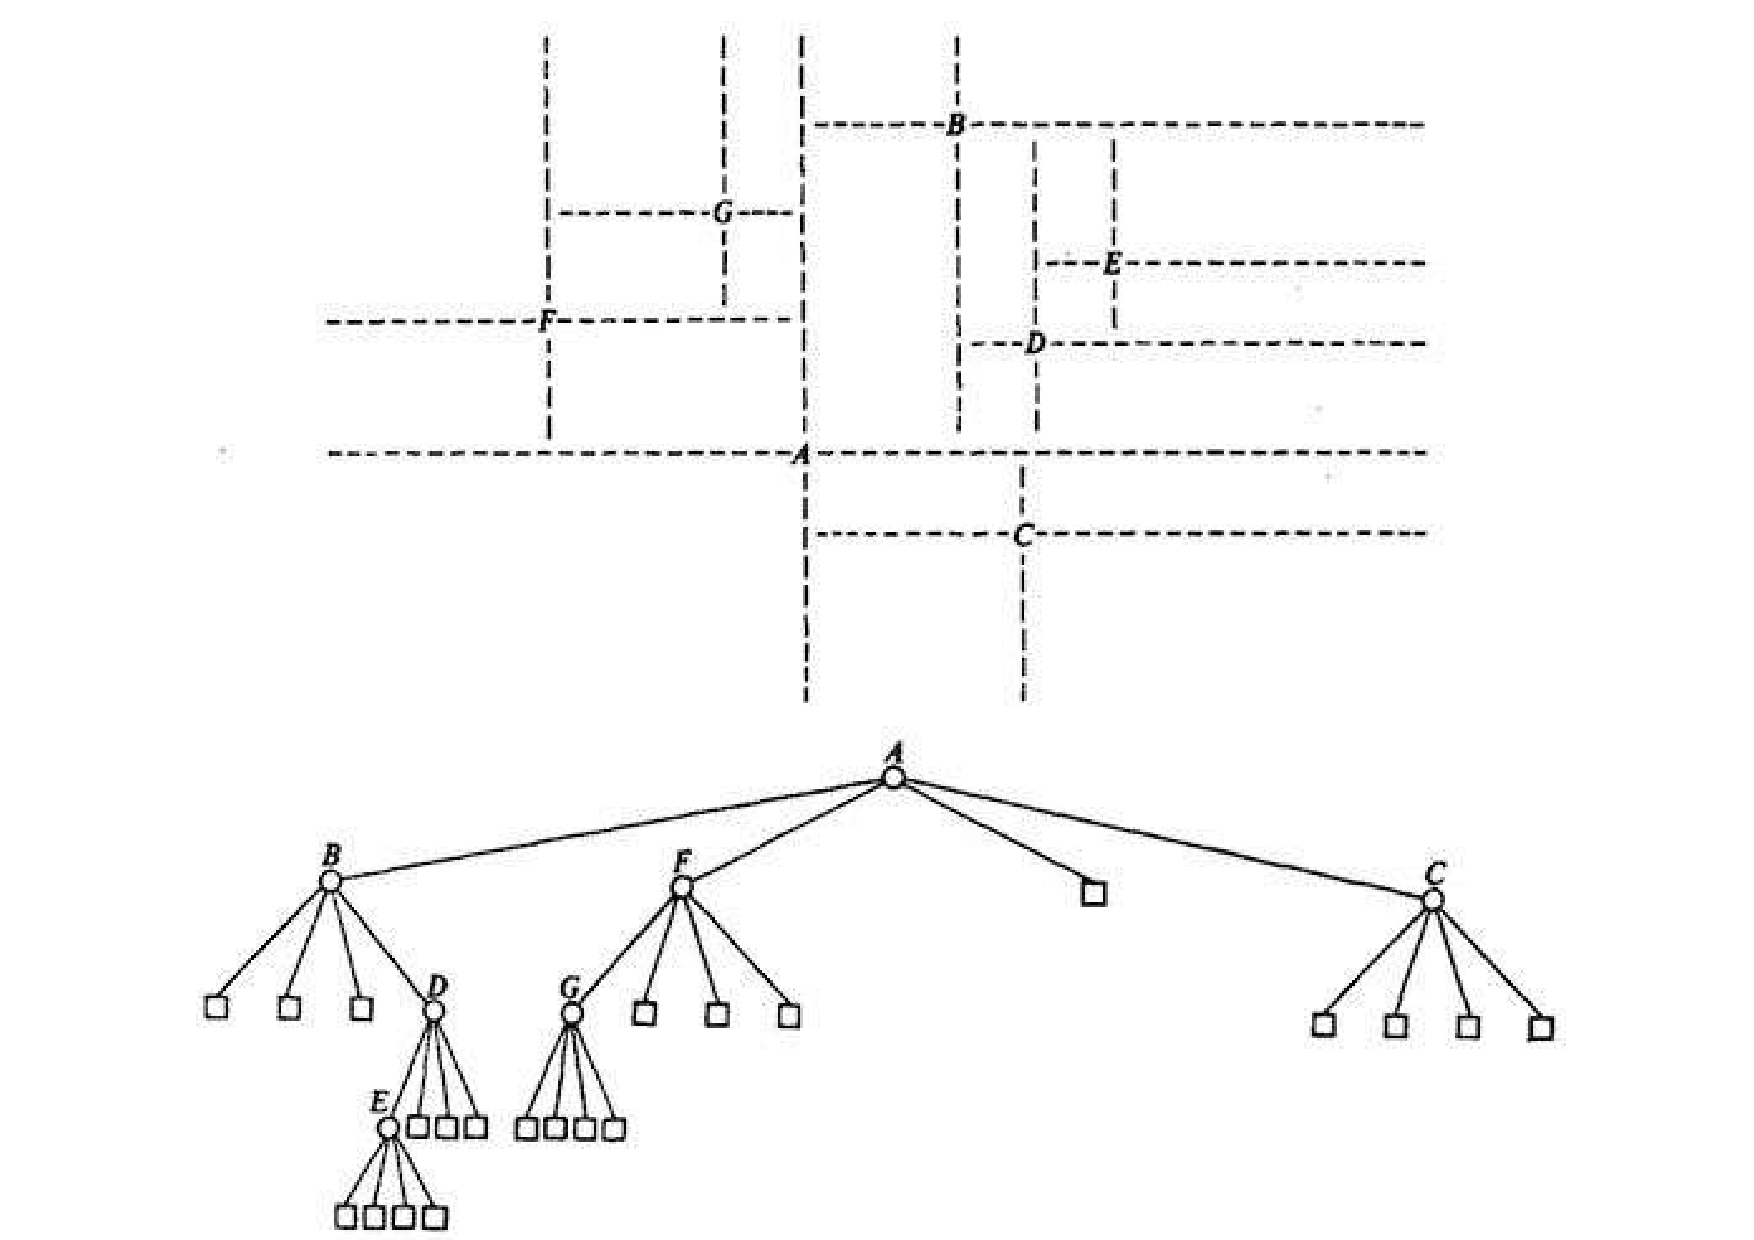
\includegraphics[width=\linewidth]{figures/quad-tree.pdf}
                \caption{Representación gráfica del árbol Quadtree \cite{finkel_bentley_quadtree}}
                \label{fig:tree_representation_figure}
            \end{figure}\\
        \subsection{Trabajos relacionados}
            El algoritmo es muy empleado en ciertas áreas de la computación como el procesamiento de imágenes, los Quad Trees facilitan la compresión y manipulación al dividir la imagen en regiones homogéneas, permitiendo una representación más compacta y eficiente. En el campo de visión computacional también tiene mucha utilidad, a modo de ejemplo se tiene el estudio de Miguel González Mendoza \cite{mendoza_advances} que explica como los sensores de profundidad ofrecen nuevas oportunidades para aplicaciones de realidad aumentada o sistemas interactivos que requieran del cuerpo humano para realizar alguna acción, entonces en su investigación emplea Quad Trees para reducir el espacio de búsqueda de los algoritmos de agrupamiento, reduciendo las dimensiones elevadas de búsqueda y eliminar los espacios vacíos reduciendo la cantidad de búsquedas.

        \subsection{Segmentación basada en Quad Tree}
            Otro ejemplo, es la segmentación basada en Quad Tree para la detección de regiones homogéneas dentro de una imagen. Su enfoque se basa en tres componentes principales:
            \begin{itemize}
                \item Suavizado con Quad Tree (Quad-tree smoothing)
                \item Clasificación (Classification)
                \item Estimación de bordes (Boundary estimation)
            \end{itemize}
            A través de estos tres pasos, el algoritmo busca reducir el ruido, clasificar los píxeles de la imagen de manera eficiente y refinar las fronteras entre regiones segmentadas.
            El primer componente, \textbf{Quad-tree smoothing}, aplica un proceso de suavizado jerárquico sobre la imagen. Cada nivel del Quad Tree representa una versión más suavizada de la imagen, en la que cada nodo se obtiene promediando los valores de sus cuatro nodos hijos en el nivel anterior. Este procedimiento permite reducir la variabilidad de la calidad sin perder información estructural importante.
            En el segundo componente de \textbf{Clasificación}, la imagen en el nivel más alto del Quad Tree se segmenta utilizando un algoritmo de clustering del centroide local. Este método no requiere información previa sobre el número de clases y agrupa los píxeles según sus estadísticas de nivel de gris, el algoritmo se ejecuta con diferentes tamaños de ventana, aceptando el resultado cuando las segmentaciones obtenidas son consistentes.
            El tercer componente, \textbf{Boundary estimation}, se encarga de refinar los bordes de las regiones segmentadas mediante un proceso descendente dentro de la jerarquía del Quad Tree. Para ello, se define una región de borde donde la clasificación no es completamente segura. Los nodos fuera de esta región mantienen la clasificación del nivel superior, mientras que los nodos dentro del área se refinan utilizando un filtro de suavizado y un criterio de distancia mínima, reduciendo el ancho de los bordes progresivamente, hasta obtener la mayor resolución de la imagen. \cite{spann_wilson_quadtree}
%----------------------------------------------------------
%----------------------------------------------------------
% REAL CASES
%----------------------------------------------------------
    \section{Operaciones}
        El quadtree se implementa como una generalización multidimensional de un árbol binario de búsqueda. En dos dimensiones, cada punto de datos se representa como un nodo en un quadtree en forma de un registro de tipo \textbf{nodo} que contiene siete campos. Los primeros cuatro campos contienen punteros a los cuatro hijos del nodo correspondientes a las direcciones (es decir, cuadrantes) NW, NE, SW y SE. Si $P$ es un puntero a un nodo y $i$ es un cuadrante, entonces estos campos se referencian como $\text{SON}(P, i)$. Podemos determinar el cuadrante específico en el que se encuentra un nodo, digamos $p$, en relación con su padre mediante el uso de la función $\text{SONTYPE}(P)$, que tiene un valor de $i$ si $\text{SON}(\text{FATHER}(P),i) = P$.
        $\text{XCOORD}$ e $\text{YCOORD}$ contienen los valores de las coordenadas $x$ e $y$, respectivamente, del punto de datos. El campo $\text{NAME}$ contiene información descriptiva sobre el nodo (por ejemplo, el nombre de la ciudad). Suponemos que cada punto de datos es único. Si una aplicación permite colisiones (es decir, varios puntos de datos con las mismas coordenadas), entonces la estructura de datos podría contener un campo adicional en el que se almacenaría un puntero a una lista de colisiones de desbordamiento. Se podría argumentar que dedicar un campo adicional a un evento poco frecuente, como una colisión, desperdicia almacenamiento; sin embargo, sin él, requeriríamos un procedimiento de inserción de nodos considerablemente más complicado.

        \subsection{Inserción}
            Los registros se insertan en árboles cuaternarios de puntos de una manera similar a la que se hace para los árboles de búsqueda binaria. En esencia, buscamos el registro deseado en función de sus coordenadas \(x\) e \(y\). En cada nodo se realiza una comparación mediante el uso del procedimiento \texttt{PT\_COMPARE} y se elige el subárbol apropiado para la siguiente prueba. Al llegar al final del árbol (es decir, cuando se encuentra un puntero \texttt{NIL}), encontramos la ubicación donde se insertará el registro. La inserción real se logra mediante el uso del procedimiento \texttt{PT\_INSERT}.
        
            Para manejar los puntos de datos que se encuentran directamente en una de las líneas del cuadrante que emanan de un punto de datos, digamos \(P\), adoptamos las mismas convenciones utilizadas para el método de cuadrícula; los límites inferior e izquierdo de cada bloque están cerrados, mientras que los límites superior y derecho de cada bloque están abiertos.\cite{samet_spatial_structures}
            \begin{algorithm}
                \caption{PT\_COMPARE(P, R)}
                \begin{algorithmic}[1]
                    \Statex \textbf{Input:} Pointer nodes $P$, $R$
                    \Statex \textbf{Output:} Quadrant where node $P$ belongs in the quadtree rooted at $R$
                    \If {$XCOORD(P) < XCOORD(R)$}
                    \If {$YCOORD(P) < YCOORD(R)$}
                    \State \Return 'SW'
                    \Else
                    \State \Return 'NW'
                    \EndIf
                    \Else
                    \If {$YCOORD(P) < YCOORD(R)$}
                    \State \Return 'SE'
                    \Else
                    \State \Return 'NE'
                    \EndIf
                    \EndIf
                \end{algorithmic}
            \end{algorithm}
            \begin{algorithm}
                \caption{PT\_INSERT(P, R)}
                \begin{algorithmic}[1]
                    \Statex \textbf{Input:} Pointer node $P$, reference pointer node $R$
                    \Statex \textbf{Output:} Insert node $P$ into the point quadtree rooted at $R$
                    \If {$R = \text{null}$}
                    \State $R \gets P$ \Comment{The tree at $R$ is initially empty}
                    \Else
                    \State $T \gets R$
                    \While {not($T = \text{null}$) and not(EQUAL\_COORD$(P, T)$)}
                    \State $F \gets T$ \Comment{Remember the father}
                    \State $Q \gets$ PT\_COMPARE$(P, T)$
                    \State $T \gets$ SON$(T, Q)$
                    \EndWhile
                    \If {$T = \text{null}$}
                    \State SON$(F, Q) \gets P$ \Comment{$P$ is not already in the tree}
                    \EndIf
                    \EndIf
                \end{algorithmic}
            \end{algorithm}
            
            
        \subsection{Búsqueda(punto exacto)}
            El siguiente algoritmo realiza la búsqueda de un punto exacto dentro de un árbol cuaternario (Quad Tree). Dado un nodo raíz y un punto objetivo, la función determina si el punto está presente en la estructura. Tiene como entradas a $Q$: Nodo raíz del Quad Tree y a $p$: Punto a buscar en el Quad Tree. Como salida: Retorna el valor asociado al punto $p$ si se encuentra en el Quad Tree, o Retorna $NULL$ si el punto $p$ no está presente.
            Internamente en el algoritmo, si el nodo $Q$ es $NULL$, el punto no se encuentra en el Quad Tree, por lo que se retorna $NULL$. Si el punto $p$ coincide con la coordenada almacenada en $Q$, se retorna el valor asociado a $Q$. Se determina en qué cuadrante del área delimitada por $Q$ se encuentra $p$: \cite{samet_spatial_structures}
            \begin{itemize}
                \item \textbf{Noreste (NE) $\rightarrow$ Se recurre al subárbol $Q.NE$.}
                \item \textbf{Noroeste (NW) $\rightarrow$ Se recurre al subárbol $Q.NW$.}
                \item \textbf{Sureste (SE) $\rightarrow$ Se recurre al subárbol $Q.SE$.}
                \item \textbf{Suroeste (SW) $\rightarrow$ Se recurre al subárbol $Q.SW$.}
            \end{itemize}
            Si $p$ no está en ninguno de los subárboles, se retorna $NULL$.
            \begin{algorithm}
                \caption{SEARCH(Q, p)}
                \begin{algorithmic}[1]
                \Statex \textbf{Input:} A Quad Tree node $Q$ and a point $p$
                \Statex \textbf{Output:} The value associated with point $p$ or \textbf{NULL} if not found
                
                \If {$Q = \text{NULL}$} 
                    \State \Return \textbf{NULL} \Comment{The point is not in the tree}
                \EndIf
                
                \If {$Q.\text{coordinate} = p$}
                    \State \Return $Q.\text{value}$ \Comment{Exact point found}
                \EndIf
                
                \If {$p$ is contained in the NE quadrant of $Q.\text{boundary}$}
                    \State \Return SEARCH($Q.\text{NE}$, $p$)
                \EndIf
                
                \If {$p$ is contained in the NW quadrant of $Q.\text{boundary}$}
                    \State \Return SEARCH($Q.\text{NW}$, $p$)
                \EndIf
                
                \If {$p$ is contained in the SE quadrant of $Q.\text{boundary}$}
                    \State \Return SEARCH($Q.\text{SE}$, $p$)
                \EndIf
                
                \If {$p$ is contained in the SW quadrant of $Q.\text{boundary}$}
                    \State \Return SEARCH($Q.\text{SW}$, $p$)
                \EndIf
                
                \State \Return \textbf{NULL} \Comment{The point is not in the Quad Tree}
                
                \end{algorithmic}
            \end{algorithm}
            \subsubsection{Complejidad Computacional}
                La complejidad del algoritmo de búsqueda de un punto exacto en un Quad Tree balanceado con $N$ puntos es aproximadamente $O(\log N)$, ya que la búsqueda se reduce a un único subárbol en cada nivel. En el peor caso (árbol degenerado), la complejidad puede ser $O(N)$.
        \subsection{Búsqueda por Rango}
            El siguiente algoritmo realiza una búsqueda de rango en un árbol Quad Tree y devuelve todos los puntos dentro de una región rectangular determinada. Tiene como entradas a $Q$: Nodo raíz del árbol cuaternario y a $R$: Región de búsqueda rectangular. Y arroja como salida una lista de puntos dentro de la región $R$.
            Recorriendo el algoritmo, si $Q$ es $NULL$, no hay puntos para buscar, por lo que la función finaliza. En cambio, si $Q.coordinate$ está dentro de la región de búsqueda $R$, se agrega a la lista de resultados. La función verifica recursivamente cada subárbol ($NE$, $NW$, $SE$, $SW$) solo si: el subárbol correspondiente no es $NULL$, el límite del subárbol interseca la región de búsqueda $R$ (para evitar una recursión innecesaria). El algoritmo continúa recursivamente hasta que se han encontrado todos los puntos relevantes.\cite{samet_spatial_structures}
            \begin{algorithm}
                \caption{RANGE\_SEARCH(Q, R, result)}
                \begin{algorithmic}[1]
                    \Statex \textbf{Input:} A Quad Tree node $Q$, a rectangular search region $R$, and a list $result$
                    \Statex \textbf{Output:} A list of points contained within $R$
                    
                    \If {$Q = \text{NULL}$}
                        \State \Return \Comment{No points to search}
                    \EndIf
                    
                    \If {$Q.\text{coordinate}$ is inside $R$}
                        \State Append $Q.\text{coordinate}$ to $result$ \Comment{Point is within the range}
                    \EndIf
                    
                    \If {$Q.\text{NE} \neq \text{NULL}$ and $Q.\text{NE}.\text{boundary}$ intersects $R$}
                        \State RANGE\_SEARCH($Q.\text{NE}$, $R$, $result$)
                    \EndIf
                    
                    \If {$Q.\text{NW} \neq \text{NULL}$ and $Q.\text{NW}.\text{boundary}$ intersects $R$}
                        \State RANGE\_SEARCH($Q.\text{NW}$, $R$, $result$)
                    \EndIf
                    
                    \If {$Q.\text{SE} \neq \text{NULL}$ and $Q.\text{SE}.\text{boundary}$ intersects $R$}
                        \State RANGE\_SEARCH($Q.\text{SE}$, $R$, $result$)
                    \EndIf
                    
                    \If {$Q.\text{SW} \neq \text{NULL}$ and $Q.\text{SW}.\text{boundary}$ intersects $R$}
                        \State RANGE\_SEARCH($Q.\text{SW}$, $R$, $result$)
                    \EndIf
                    
                    \State \Return \Comment{Result list is updated recursively}
                
                \end{algorithmic}
            \end{algorithm}
            
        \subsubsection{Complejidad Computacional}
                La complejidad de tiempo del peor caso depende de la cantidad de puntos dentro de la región de búsqueda:
                \begin{itemize}
                \item \textbf{Mejor caso:} $O(\log N)$ (para árboles dispersos donde la recursión es mínima).
                \item \textbf{Peor caso:} $O(N)$ (si todos los puntos están dentro de la región de búsqueda y necesitan ser verificados).
                \end{itemize}
        \subsection{Optimización Mediante Poda}
                La \textbf{poda en Quad Trees} optimiza la búsqueda descartando regiones completas que \textbf{no intersectan} con la zona de búsqueda, evitando exploraciones innecesarias. Esto reduce la cantidad de nodos visitados, mejorando la eficiencia y permitiendo que la búsqueda se realice en \textbf{O(logN)} en casos balanceados.

                \textbf{Para realizar la poda debemos hacer lo siguiente:}
                \begin{enumerate}
                    \item \textbf{Verificar si el nodo actual es NULL}
                    \begin{itemize}
                        \item Si el nodo \textbf{no existe}, se retorna inmediatamente sin explorar más.
                    \end{itemize}
                    
                    \item \textbf{Comprobar si la región del nodo intersecta con la región de búsqueda}
                    \begin{itemize}
                        \item Si el área representada por el nodo \textbf{NO INTERSECTA} con la región de búsqueda, \textbf{se descarta todo el subárbol}, evitando llamadas recursivas innecesarias.
                    \end{itemize}
                    
                    \item \textbf{Si el nodo contiene un punto, verificar si está dentro de la región de búsqueda}
                    \begin{itemize}
                        \item Si el punto está dentro del rango, \textbf{se añade al resultado}.
                    \end{itemize}
                    
                    \item \textbf{Si la región del nodo sí intersecta con la búsqueda, continuar la recursión solo en los subárboles relevantes}
                \end{enumerate}
    %----------------------------------------------------------
%----------------------------------------------------------
% CONCLUTIONS
%----------------------------------------------------------        
    \section{Análisis comparativo entre Quad Tree y K-D Tree}
        \subsection*{K-D Tree:}
            Un K-D Tree es una estructura de datos en forma de árbol binario donde cada nodo es un punto en un espacio k-dimensional. Cada nivel del árbol compara una dimensión diferente, alternando entre ellas en cada nivel de profundidad. Las aplicaciones de los K-D Trees incluyen búsquedas multidimensionales, como búsquedas de rango y de vecinos más cercanos, así como compresión de imágenes.
        
        \subsection*{Inserción:}
            \begin{itemize}
            \item \textbf{Número de puntos de datos:} Se observa que, en teoría, el tiempo de construcción en el peor de los casos para ambos árboles es $O(n \log n)$, pero en promedio es $O(n)$. En la práctica, la construcción de Quad Trees requiere más tiempo que la de K-D Trees debido a la mayor profundidad de recorrido por inserción en los Quad Trees.
            \begin{figure}[h]
                \centering
                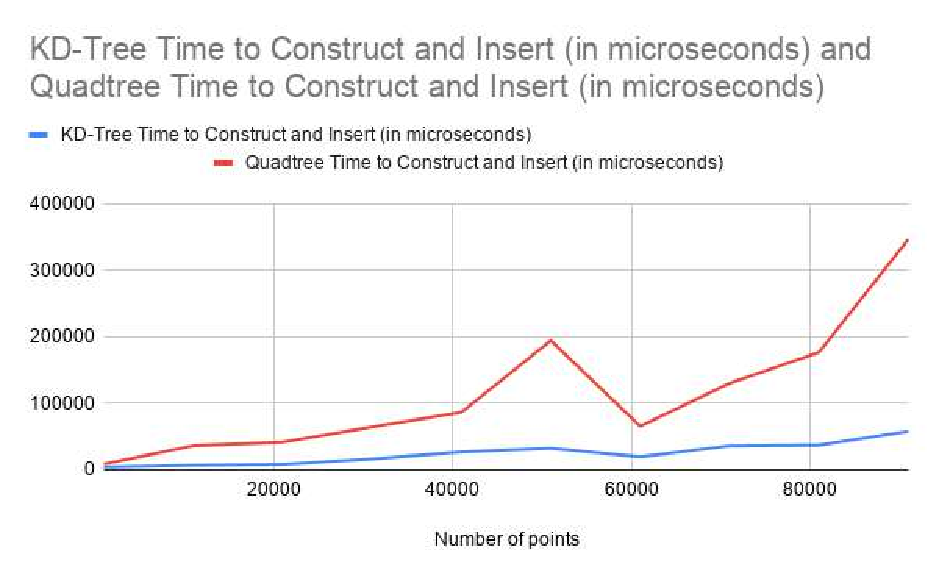
\includegraphics[width=\linewidth]{figures/Insertion.pdf}
                \caption{Inserción por puntos\cite{amay12_spatialsearch}}
                \label{fig:insertion_p_p_figure}
            \end{figure}
            \item \textbf{Distribución de densidad de puntos:} A medida que aumenta la densidad de puntos en una región específica del plano 2D, disminuye el tiempo promedio de construcción e inserción para ambos árboles, ya que es menos probable que se creen nuevos nodos hijos.
            \end{itemize}
            \begin{figure}[h]
                \centering
                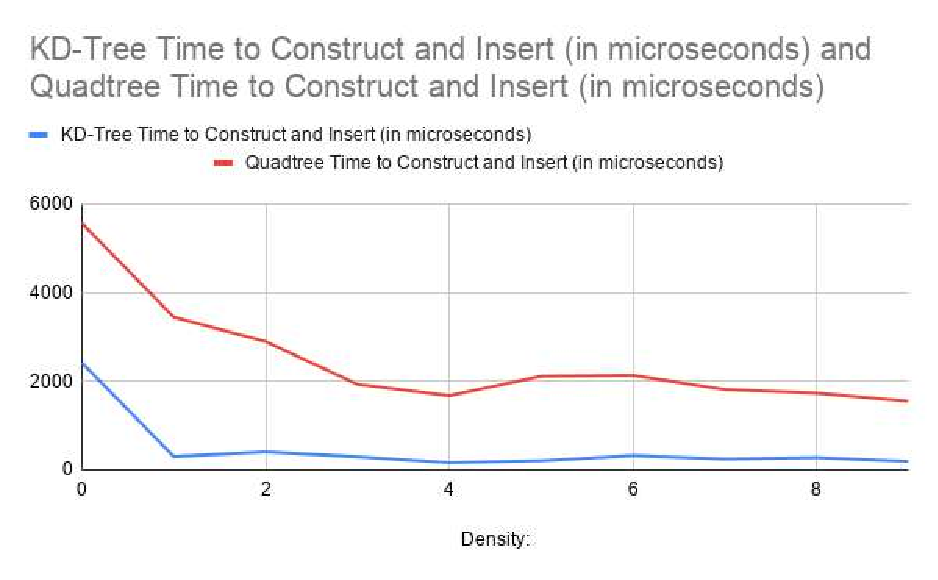
\includegraphics[width=\linewidth]{figures/insertion2.pdf}
                \caption{Inserción por densidad\cite{amay12_spatialsearch}}
                \label{fig:insertion_p_d_figure}
            \end{figure}
        \subsection*{Búsqueda:}
            \begin{itemize}
            \item \textbf{Número de puntos de datos:} Se encuentra que los Quad Trees son más rápidos que los K-D Trees en operaciones de búsqueda a medida que aumenta el tamaño de los datos. Esto se debe a que los Quad Trees tienen un factor de ramificación de 4, lo que reduce la profundidad del árbol en comparación con los K-D Trees, que tienen un factor de ramificación de 2.\\
                \begin{figure}[h]
                \centering
                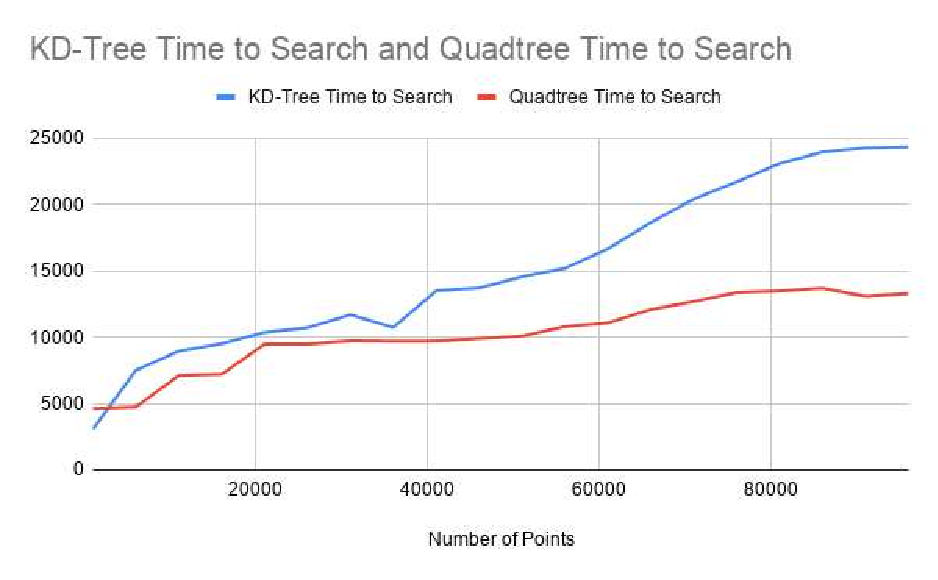
\includegraphics[width=\linewidth]{figures/Search1.pdf}
                \caption{Búsqueda por puntos\cite{amay12_spatialsearch}}
                \label{fig:search_p_p_figure}
            \end{figure}
            \item \textbf{Distribución de densidad de puntos:} Con una distribución dispersa de puntos, los Quad Trees superan a los K-D Trees en términos
            de tiempo de búsqueda. Sin embargo, a medida que la densidad aumenta, el rendimiento relativo de los Quad Trees sigue siendo mejor, excepto en casos donde el Quad Tree está sesgado, lo que puede llevar a una complejidad temporal promedio de $O(n)$.\\
            \begin{figure}[h]
                \centering
                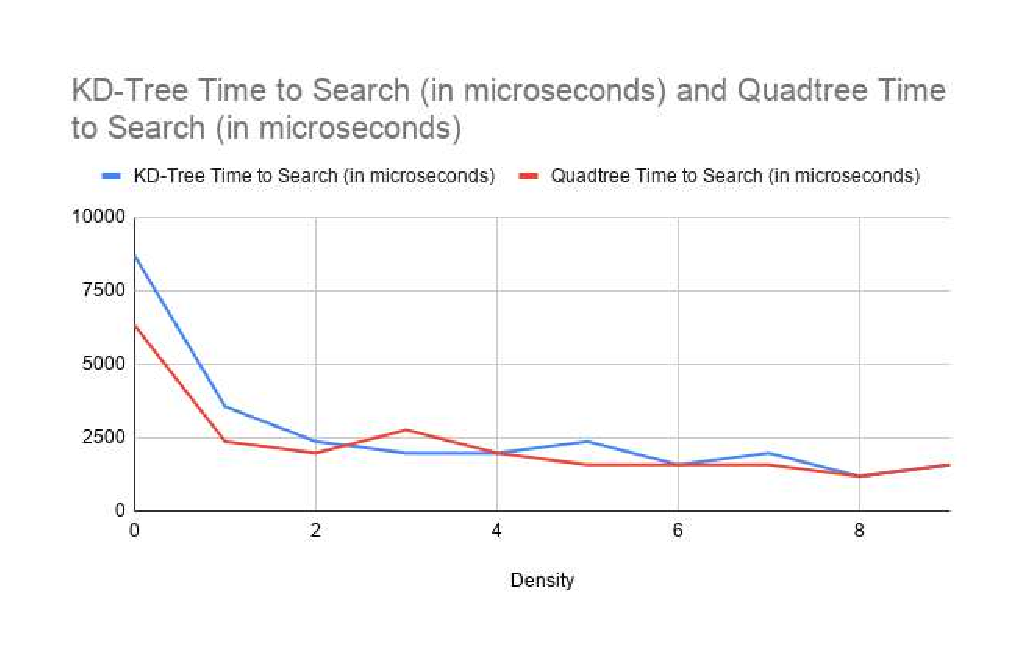
\includegraphics[width=\linewidth]{figures/Search2-density.pdf}
                \caption{Búsqueda por densidad \cite{amay12_spatialsearch}}
                \label{fig:search_p_d_figure}
            \end{figure}
        \end{itemize}
    
    \subsection*{Búsqueda del vecino más cercano:}
        Los K-D Trees son muy eficientes en la búsqueda del vecino más cercano, con una complejidad temporal promedio de $O(\log N)$, siempre que el árbol no esté altamente desequilibrado. Por otro lado, los Quad Trees no están optimizados para este tipo de búsqueda y pueden requerir más tiempo para calcular el vecino más cercano.\\
\section{Aplicaciones Prácticas}
    \subsection[Detección de Bordes usando Quad Tree]{Detección de Bordes usando Quad Tree}

    Un Quad Tree es una estructura de datos que divide un espacio 2D en cuatro cuadrantes iguales. Cada cuadrante puede subdividirse recursivamente, lo que permite una representación jerárquica de los datos espaciales. Esta estructura es especialmente útil para aplicaciones como la detección de bordes, ya que permite manejar grandes volúmenes de datos de manera eficiente al reducir la complejidad computacional.
    
        \subsubsection{Detección de Bordes}
        
        La detección de bordes es un proceso crítico en el análisis de imágenes, ya que permite identificar las transiciones entre diferentes regiones de una imagen. Un método comúnmente utilizado para la detección de bordes es el algoritmo de Canny, que se puede integrar con Quad Trees para mejorar la eficiencia y precisión en la segmentación como se puede observar en la Figura~\ref{fig:deteccion_figure}
        
        \subsubsection{Pasos para Implementar Detección de Bordes con Quad Trees}
        
        \begin{enumerate}
            \item \textbf{División Inicial:} Comienza dividiendo la imagen en cuadrantes utilizando el Quad Tree. Esta división permite enfocarse en áreas más pequeñas y manejables.
            
            \item \textbf{Aplicación del Algoritmo de Detección de Bordes:} Para cada cuadrante, aplica el algoritmo de Canny o cualquier otro método adecuado para detectar bordes. Esto implica suavizar la imagen con un filtro Gaussiano y luego aplicar técnicas para encontrar los contornos.
            
            \item \textbf{Segmentación:} Una vez que se han detectado los bordes, se pueden segmentar los cuadrantes que contienen información relevante sobre los objetos en la imagen. Los cuadrantes vacíos o irrelevantes pueden ser descartados, optimizando así el proceso.
            
            \item \textbf{Manejo de Transiciones:} Es fundamental manejar adecuadamente las transiciones en los bordes, ya que esto puede afectar la calidad del análisis. Se deben establecer reglas para asegurar que los elementos generados sean válidos y representen correctamente el borde del objeto.
            
            \item \textbf{Revisión y Refinamiento:} Finalmente, revisa los cuadrantes resultantes y refina la segmentación según sea necesario. Esto puede incluir la eliminación de elementos inválidos o la mejora de los ángulos y formas detectadas.
        \end{enumerate}
        
        \subsubsection{Ventajas del Uso de Quad Trees en Detección de Bordes}
        
        \begin{itemize}
            \item \textbf{Eficiencia Computacional:} Al dividir el espacio en cuadrantes, se reduce la cantidad de datos a procesar en cada paso.
            
            \item \textbf{Escalabilidad:} La estructura permite manejar imágenes grandes sin comprometer el rendimiento.
            
            \item \textbf{Flexibilidad:} Se puede adaptar a diferentes tipos de imágenes y requisitos específicos del análisis.
        \end{itemize}
        
        En resumen, la detección de bordes utilizando Quad Trees combina la eficiencia estructural con técnicas avanzadas de procesamiento de imágenes, lo que resulta en un método poderoso para segmentar y analizar objetos dentro de imágenes digitales.
        \begin{figure}[h]
            \centering
            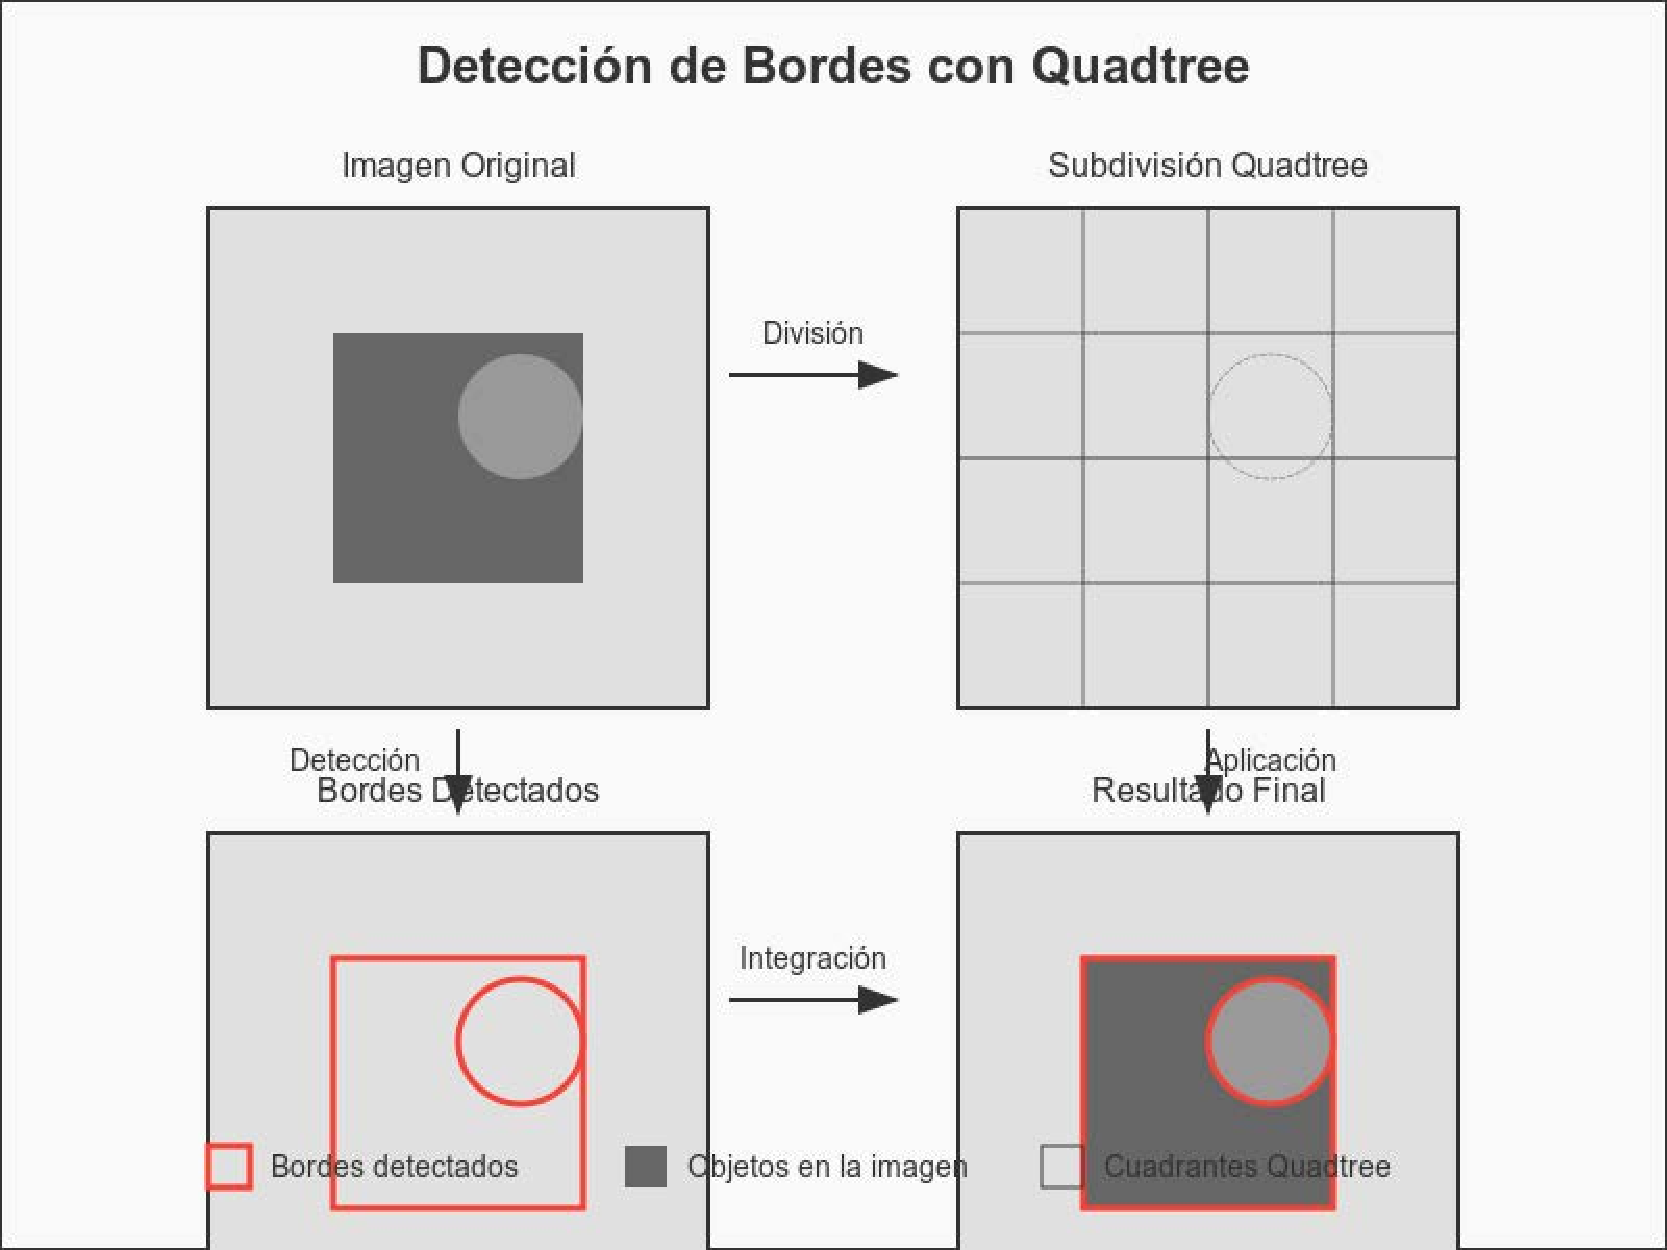
\includegraphics[width=\linewidth]{figures/edge-detection.pdf}
            \caption{Representación grafica de detección de bordes} 
            \label{fig:deteccion_figure}
        \end{figure}
    \subsection[Detección de Colisiones]{Detección de Colisiones}

        La detección de colisiones usando Quad Trees es una técnica eficiente para manejar la interacción entre múltiples objetos en un entorno 2D, especialmente en aplicaciones como videojuegos.

        Un Quad Tree es una estructura de datos jerárquica que divide un espacio bidimensional en cuatro cuadrantes o nodos hijos. Cada nodo puede contener objetos y, si el número de objetos en un cuadrante excede un límite predefinido, ese cuadrante se subdivide nuevamente en cuatro partes. Este enfoque permite gestionar grandes cantidades de objetos sin necesidad de verificar cada posible colisión entre ellos, lo que sería computacionalmente costoso.

    \subsubsection{Funcionamiento}
    \begin{itemize}
        \item \textbf{División del espacio:} El espacio se divide inicialmente en cuatro cuadrantes. Cada cuadrante puede contener múltiples objetos.
        
        \item \textbf{Subdivisión:} Si un cuadrante contiene más de un número determinado de objetos (por ejemplo, 10), se subdivide en cuatro nuevos cuadrantes. Este proceso puede repetirse hasta alcanzar una profundidad máxima deseada.
        
        \item \textbf{Comprobación de colisiones:} Al realizar la detección de colisiones, cada objeto solo necesita verificar colisiones con otros objetos dentro de su mismo cuadrante o los cuadrantes adyacentes, reduciendo significativamente el número de verificaciones necesarias; Como se puede visualizar en la Figura~\ref{fig:colision_figure}.
    \end{itemize}

    \subsubsection{Ventajas del uso de Quad Trees}
    \begin{itemize}
        \item \textbf{Reducción del costo computacional:} En lugar de realizar $O(n^2)$ comprobaciones (donde $n$ es el número de objetos), el uso de Quad Trees puede reducir este número a $O(n\log n)$ o incluso menos, dependiendo de la distribución espacial de los objetos.
        
        \item \textbf{Eficiencia en escenarios dinámicos:} En entornos donde los objetos se mueven constantemente, los Quad Trees pueden actualizarse rápidamente al mover objetos entre cuadrantes según sea necesario.
        
        \item \textbf{Facilidad para manejar diferentes escalas:} Los Quad Trees son útiles para manejar diferentes tamaños y formas de objetos, permitiendo que las comprobaciones sean más precisas.
    \end{itemize}

    \subsubsection{Implementación práctica}
    Para implementar un Quad Tree para la detección de colisiones:

        \begin{itemize}
            \item \textbf{Definir la estructura del nodo:} Cada nodo debe contener información sobre su área (rectángulo delimitador), una lista de objetos y referencias a sus nodos hijos.
            
            \item \textbf{Método para insertar objetos:} Implementar un método que coloque un objeto en el nodo correspondiente y que subdivida el nodo si es necesario.
            
            \item \textbf{Método para comprobar colisiones:} Crear una función que verifique las colisiones solo con los objetos dentro del mismo nodo o nodos adyacentes.
            
            \item \textbf{Actualizar posiciones:} Al mover objetos, se debe actualizar su posición en el Quad Tree para asegurar que siempre estén en el nodo correcto.
        \end{itemize}
        \begin{figure}[H]
            \centering
            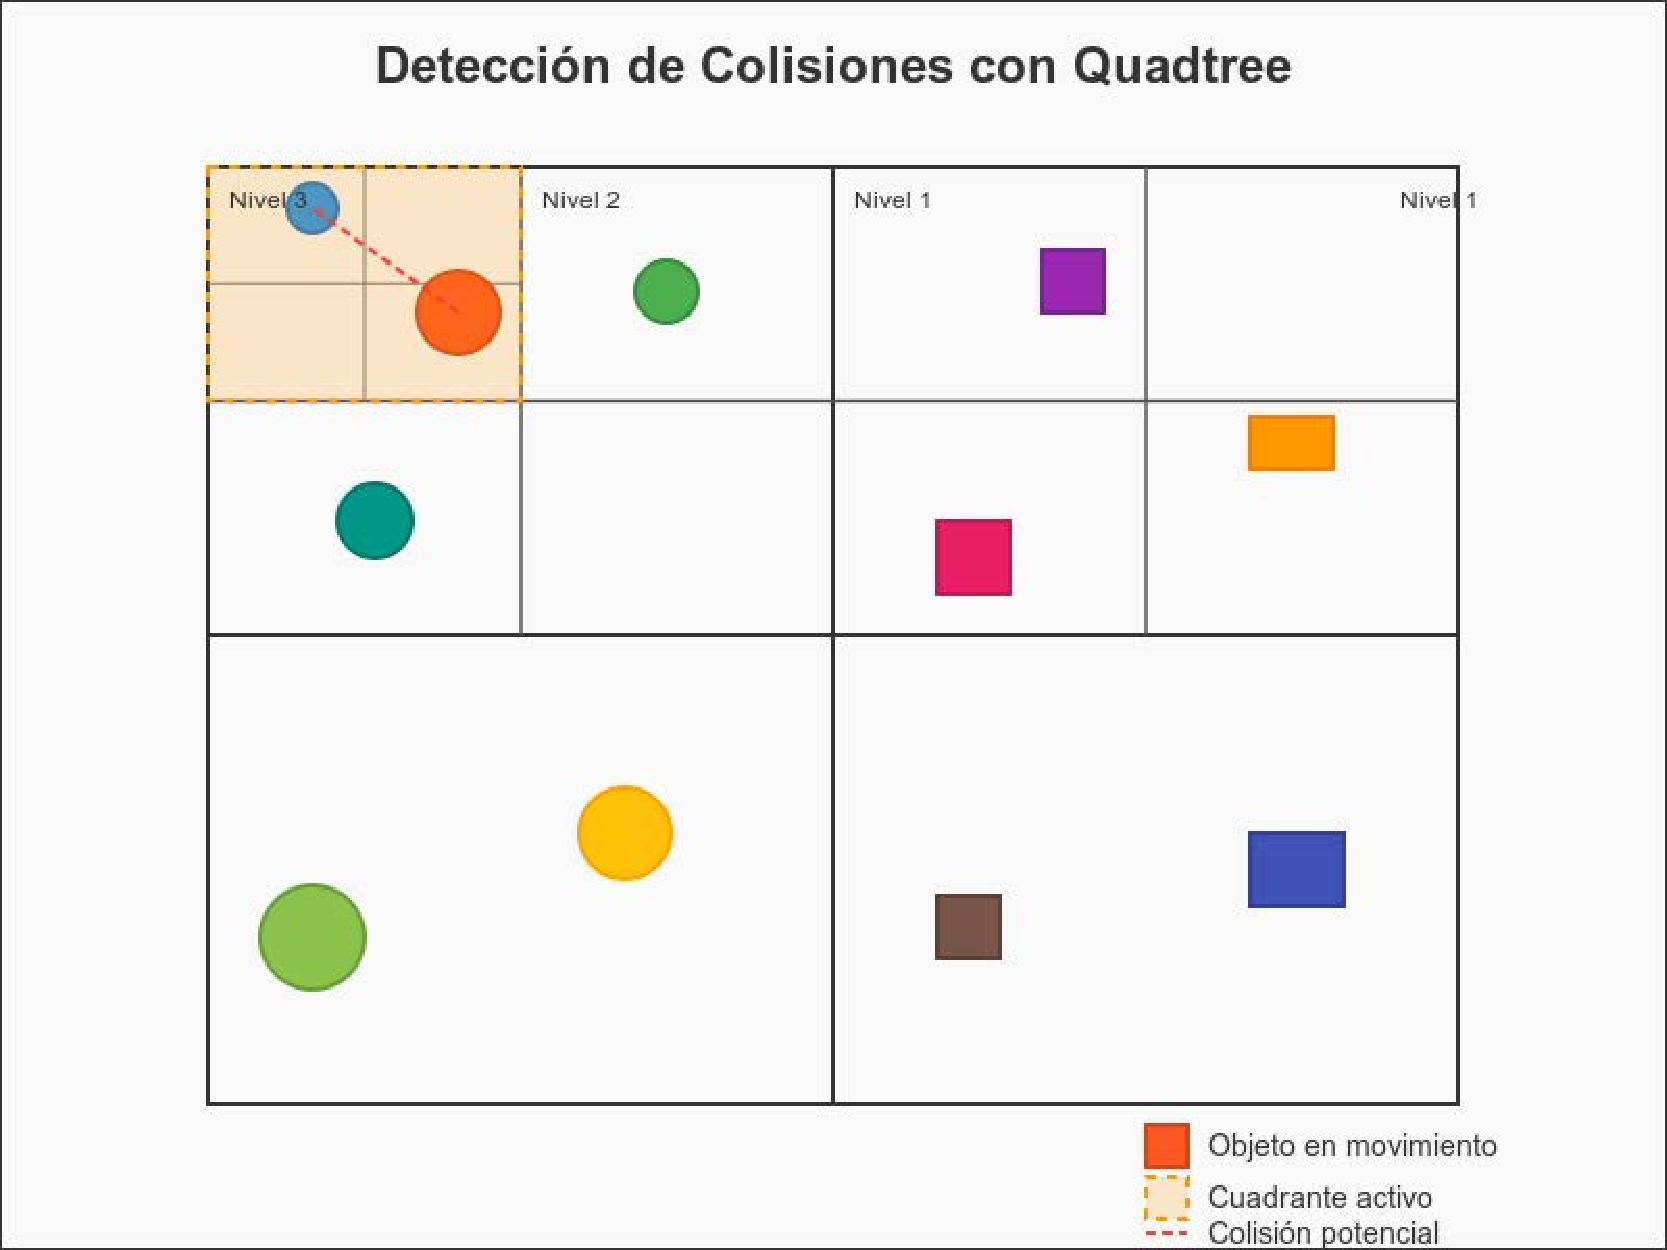
\includegraphics[width=\linewidth]{figures/quadtree-collision.pdf}
            \caption{Representación grafica de colisiones} 
            \label{fig:colision_figure}
        \end{figure}
    
    
\section{Conclusiones}

    \begin{itemize}
        \item Es uno de las mejores estructuras de datos para almacenar grandes volumenes de información.
        \item La segmentación basada en Quad Tree destaca por su capacidad para reducir el ruido, clasificar eficientemente las regiones homogéneas y refinar los bordes de las imágenes, mejorando la precisión sin comprometer el rendimiento. Por esta razón, esta estructura continúa siendo una herramienta clave para el manejo eficiente de información en escenarios de alto volumen de datos.
        \item El Quad Tree es una estructura poderosa para organizar datos espaciales. Sus algoritmos de inserción y búsqueda son eficientes en casos balanceados, con $O(\log N)$, pero pueden degradarse a $O(N)$ en situaciones desbalanceadas.
        \item El uso de poda mejora el rendimiento, descartando regiones completas del espacio durante las búsquedas.
        \item Es una opción superior a estructuras lineales para manejar datos en 2D, especialmente en aplicaciones como GIS, gráficos y videojuegos.
        \item Quad Trees son más eficientes que K-D Trees para búsquedas espaciales (por rango o región) cuando se realizan consultas frecuentes debido a la poda efectiva que reduce regiones exploradas innecesariamente.
        \item K-D Trees son superiores en operaciones como búsqueda del vecino más cercano y en la construcción rápida del árbol, especialmente cuando las consultas espaciales son menos frecuentes y se busca eficiencia en la inserción y construcción inicial del índice.\\
    \end{itemize}

\defbibheading{bibliography}{\section*{Referencias}}
\printbibliography

%----------------------------------------------------------
% CONTENTS
%----------------------------------------------------------
\renewcommand{\contentsname}{Tabla de Contenidos}
\tableofcontents
\linenumbers
%----------------------------------------------------------

% \printbibliography

%----------------------------------------------------------    

\end{document}